%!TEX root = main.tex

\section{Definitions and key notation}\label{sec:dfin}

We use three notations for working with probability theory. The ``elementary'' notation makes use of regular symbolic conventions (functions, products, sums, integrals, unions etc.) along with the expectation operator $\mathbb{E}$. This is the most flexible notation which comes at the cost of being verbose and difficult to read. Secondly, we use a semi-formal string diagram notation extending the formal diagram notation for symmetric monoidal categories \cite{selinger_survey_2010}. Objects in this diagram refer to stochastic maps, and by interpreting diagrams as symbols we can, in theory, be just as flexible as the purely symbolic approach. However, we avoid complex mixtures of symbols and diagrams elements, and fall back to symbolic representations if it is called for. Finally, we use a matrix-vector product convention that isn't particularly expressive but can compactly express some common operations.

\subsection{Standard Symbols}

\begin{center}
\begin{tabular}{ |c|c|c| } 
 \hline
 Symbol & Meaning \\ 
 $[n]$& The natural numbers $\{1,...,n\}$ \\ 
 $f:a\mapsto b$ & Function definition, equivalent to $f(a):=b$\\
 Dots appearing in function arguments: $f(\cdot,\cdot,z)$ & The ``curried'' function $(x, y )\mapsto f(x,y,z)$\\
 Capital letters: $A,B, X$ & sets \\ 
 Script letters: $\mathcal{A},\mathcal{B},\mathcal{X}$ & $\sigma$-algebras on the sets $A, B, X$ respectively\\
 Script $\mathcal{G}$ & A directed acyclic graph made up of nodes $V$ and edges $E$\\
 Greek letters $\mu, \xi, \gamma$ & Probability measures\\
 $\delta_x$ & The Dirac delta measure: $\delta_x(A) = 1$ if $x\in A$ and $0$ otherwise\\
 Capital delta: $\Delta(\mathcal{E})$ & The set of all probability measures on $\mathcal{E}$\\
 Bold capitals: $\mathbf{A}$ & Markov kernel $\mathbf{A}:X\times\mathcal{Y}\to [0,1]$ (stochastic maps)\\
 Subscripted bold capitals: $\mathbf{A}_x$ & The probability measure given by the curried Markov kernel $\mathbf{A}(x,\cdot)$\\
 $A\to\Delta(\mathcal{B})$ & Markov kernel signature, treated as equivalent to $A\times \mathcal{B}\to [0,1]$\\
 $\mathbf{A}:x\mapsto \nu$ & Markov kernel definition, equivalent to $\mathbf{A}(x,B) = \nu(B)$ for all $B$\\
 Sans serif capitals: $\RV{A},\RV{X}$ & Measurable functions; we will also call them random variables\\
 $\Pi_{\RV{X}}$ & The Markov kernel associated with the function $\RV{X}$: $\Pi_{\RV{X}} \equiv a\mapsto \delta_{\RV{X}(a)}$\\
 $\mathbf{N}_{\RV{A}|\RV{B}}$ & The conditional probability (disintegration) of $\RV{A}$ given $\RV{B}$ under $\nu$\\
 $\nu \Pi_{\RV{X}}$ & The marginal distribution of $\RV{X}$ under $\nu$\\
 \hline
\end{tabular}
\end{center}

\subsection{Probability Theory}

Given a set $A$, a $\sigma$-algebra $\mathcal{A}$ is a collection of subsets of $A$ where
\begin{itemize}
	\item $A\in \mathcal{A}$ and $\emptyset\in \mathcal{A}$
	\item $B\in \mathcal{A}\implies B^C\in\mathcal{A}$
	\item $\mathcal{A}$ is closed under countable unions: For any countable collection $\{B_i|i\in Z\subset \mathbb{N}\}$ of elements of $\mathcal{A}$, $\cup_{i\in Z}B_i\in \mathcal{A}$ 
\end{itemize}

A measurable space $(A,\mathcal{A})$ is a set $A$ along with a $\sigma$-algebra $\mathcal{A}$. Sometimes the sigma algebra will be left implicit, in which case $A$ will just be introduced as a measurable space.

\paragraph{Common $\sigma$ algebras}

For any $A$, $\{\emptyset,A\}$ is a $\sigma$-algebra. In particular, it is the only sigma algebra for any one element set $\{*\}$.

For countable $A$, the power set $\mathscr{P}(A)$ is known as the discrete $\sigma$-algebra.

Given $A$ and a collection of subsets of $B\subset\mathscr{P}(A)$, $\sigma(B)$ is the smallest $\sigma$-algebra containing all the elements of $B$. 

Let $T$ be all the open subsets of $\mathbb{R}$. Then $\mathcal{B}(\mathbb{R}):=\sigma(T)$ is the \emph{Borel $\sigma$-algebra} on the reals. This definition extends to an arbitrary topological space $A$ with topology $T$.

A \emph{standard measurable set} is a measurable set $A$ that is isomorphic either to a discrete measurable space $A$ or $(\mathbb{R}, \mathcal{B}(\mathbb{R}))$. For any $A$ that is a complete separable metric space, $(A,\mathcal{B}(A))$ is standard measurable. 

Given a measurable space $(E,\mathcal{E})$, a map $\mu:\mathcal{E}\to [0,1]$ is a \emph{probability measure} if
\begin{itemize}
	\item $\mu(E)=1$, $\mu(\emptyset)=0$
	\item Given countable collection $\{A_i\}\subset\mathscr{E}$, $\mu(\cup_{i} A_i) = \sum_i \mu(A_i)$
\end{itemize}

Write by $\Delta(\mathcal{E})$ the set of all probability measures on $\mathcal{E}$.

Given a second measurable space $(F,\mathcal{F})$, a \emph{stochastic map} or \emph{Markov kernel} is a map $\mathbf{M}:E\times\mathcal{F}\to [0,1]$ such that
\begin{itemize}
	\item The map $\mathbf{M}(\cdot;A):x\mapsto \mathbf{M}(x;A)$ is $\mathcal{E}$-measurable for all $A\in \mathcal{F}$
	\item The map $\mathbf{M}_x:A\mapsto \mathbf{M}(x;A)$ is a probability measure on $F$ for all $x\in E$
\end{itemize}

Extending the subscript notation above, for $\mathbf{C}:X\times Y\to \Delta(\mathcal{Z})$  and $x\in X$ we will write $\mathbf{C}_x$ for the ``curried'' map $y\mapsto \mathbf{C}_{x,y}$.

The map $x\mapsto \mathbf{M}_x$ is of type $E\to \Delta(\mathcal{F})$. We will abuse notation somewhat to write $\mathbf{M}:E\to \Delta(\mathcal{F})$, which captures the intuition that a Markov kernel maps from elements of $E$ to probability measures on $\mathcal{F}$. Note that we ``reverse'' this idea and consider Markov kernels to map from elements of $\mathcal{F}$ to measurable functions $E\to[0,1]$, an interpretation found in \citet{clerc_pointless_2017}, but (at this stage) we don't make use of this interpretation here.

Given an indiscrete measurable space $(\{*\},\{\{*\},\emptyset\})$, we identify Markov kernels $\mathbf{N}:\{*\}\to \Delta(\mathcal{E})$ with the probability measure $\mathbf{N}_*$. In addition, there is a unique Markov kernel $\stopper{0.2}:E\to \Delta(\{\{*\},\emptyset\})$ given by $x\mapsto \delta_*$ for all $x\in E$ which we will call the ``discard'' map

\subsection{Product Notation}

We can use a notation similar to matrix-vector products to represent operations with Markov kernels. Probability measures $\mu\in \Delta(\mathcal{X})$ can be read as row vectors, Markov kernels as matrices and measurable functions $\RV{T}:Y\to T$ as column vectors. Defining $\mathbf{M}:X\to \Delta(\mathcal{Y})$ and $\mathbf{N}:Y\to \Delta(\mathcal{Z})$, the measure-kernel product $\mu \mathbf{A} (G) := \int \mathbf{A}_x (G) d\mu(x)$ yields a probability measure $\mu\mathbf{A}$ on $\mathcal{Z}$, the kernel-kernel product $\mathbf{M}\mathbf{N}(x;H)=\int_Y \mathbf{B}(y;H)d\mathbf{A}_x$ yields a kernel $\mathbf{M}\mathbf{N}:X\to \Delta(\mathcal{Z})$ and the kernel-function product $\mathbf{A}\RV{T}(x):=\int_Y \RV{T}(y) d\mathbf{A}_x$ yields a measurable function $X\to T$. Kernel products are associative \citep{cinlar_probability_2011}.

The tensor product $(\mathbf{M}\otimes \mathbf{N})(x,y;G,H) := \mathbf{M}(x;G)\mathbf{N}(y;H)$ yields a kernel $(\mathbf{M}\otimes \mathbf{N}):X\times Y\to \Delta(\mathcal{Y}\otimes\mathcal{Z})$.

\subsection{String Diagrams}

Some constructions are unwieldly in product notation; for example, given $\mu\in \Delta(\mathcal{E})$ and $\mathbf{M}:E\to (\mathcal{F})$, it is not straightforward to construct a measure $\nu\in\Delta(\mathcal{E}\otimes\mathcal{F})$ that captures the ``joint distribution'' given by $A\times B\mapsto \int_A \mathbf{M}(x;B)d\mu$. 

Such constructions can, however, be straightforwardly captured with string diagrams, a notation developed for category theoretic probability. \citet{cho_disintegration_2019} also provides an extensive introduction to the notation discussed here.

Some key ideas of string diagrams:
\begin{itemize}
	\item Basic string diagrams can always be interpreted as a mixture of kernel-kernel products and tensor products of Markov kernels
	\begin{itemize}
	\item Extended string diagrams can be interepreted as a mixture of kernel-kernel products, kernel-function products, tensor products of kernels and functions and scalar products 
	\end{itemize}
	\item String diagrams are the subject of a coherence theorem: taking a string diagram and applying a planar deformation yields a string diagram that represents the same kernel \citep{selinger_survey_2010}. This also holds for a number of additional transformations detailed below
\end{itemize}

A kernel $\mathbf{A}:X\to \Delta(\mathcal{Y})$ is written as a box with input and output wires, probability measures $\mu\in \Delta(\mathcal{X})$ are written as triangles ``closed on the left'' and measurable functions $\RV{T}:Y\to T$ as triangles ``closed on the right''.

\begin{align}
\begin{tikzpicture}
\path (0,0) coordinate (A)
++(0.5,0) node[kernel] (B) {$\mathbf{A}$}
++(0.5,0) coordinate (C);
\draw (A) -- (B) -- (C);
\end{tikzpicture}\qquad
\begin{tikzpicture}
\path (0,0) node[dist] (B) {$\mu$}
++(0.5,0) coordinate (C);
\draw (B) -- (C);
\end{tikzpicture}\qquad
\begin{tikzpicture}
\path (0,0) coordinate (A)
++(0.5,0) node[expectation] (B) {$\RV{T}$};
\draw (A) -- (B);
\end{tikzpicture}
\end{align}

We canonically regard a probability measure $\mu\in \Delta(\mathcal{E})$ to be a Markov kernel $\mu:\{*\}\to \Delta(\mathcal{E})$. This allows for the definition of ``basic'' string diagrams for which Markov kernels are the only building blocks. Such a definition isn't possible for measurable functions. Suppose by analogy with the example probability measures and try to identify a measurable function $f:E\to \mathbb{R}$ with a Markov kernel $f':E\times\{*\}\to \mathbb{R}$. For $x\in E$ we cannot generally have both $f'(x,*)=1$ and $f'(x,*)=f(x)$, and so this attempt fails. This lack of normalisation is the reason we require an ``extended'' string diagram notation if we wish to incorporate functions and expectations which allows for the representation of scalars.

\paragraph{Markov kernels with special notation}

A number of Markov kernels are given special notation distinct from the generic ``box'' representation above. These special representations facilitate intuitive graphical interpretations.

The identity kernel $\textbf{Id}:X\to \Delta(X)$ maps a point $x$ to the measure $\delta_x$ that places all mass on the same point:

\begin{align}
\textbf{Id}_x : x\mapsto \delta_x \equiv \begin{tikzpicture}\path (0,0) node (X) {$X$} + (1,0) node (X1) {$\RV{X}$}; \draw (X)--(X1); \end{tikzpicture}
\end{align}


The copy map $\splitter{0.1}:X\to \Delta(X\times X)$ maps a point $x$ to two identical copies of x:
\begin{align}
 \splitter{0.1}: x\mapsto \delta_{(x,x)} \equiv 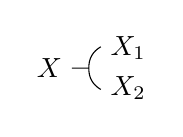
\begin{tikzpicture}
 \path (0,0) node (X) {$X$} ++ (0.5,0) coordinate (copy0) ++ (0.5,0.25) node (X1) {$\RV{X}_1$} ++(0,-0.5) node (X2) {$\RV{X_2}$};\draw (X)--(copy0) to [bend left] (X1) (copy0) to [bend right] (X2);
 \end{tikzpicture}
 \end{align} 

The discard map $\stopper{0.2}:X\to \Delta(\{*\})$ maps every input to $\delta_{*}$ which is effectively mapping every input to 1
\begin{align}
\stopper{0.2}: x\mapsto \delta_{*} \equiv \begin{tikzpicture}
 \draw[-{Rays [n=8]}] (0,0) -- (0.5,0);
\end{tikzpicture}
\end{align}

The swap map $\sigma:X\times Y\to \Delta(\mathcal{Y}\otimes\mathcal{X})$ swaps its inputs:

\begin{align}
\sigma := (x,y)\to \delta_{(y,x)} \equiv 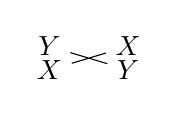
\begin{tikzpicture}
\path (0,0) node (X) {$X$}
+(1,0.3) node (X1) {$\RV{X}$}
(0,0.3) node (Y) {$Y$}
+(1,-0.3) node (Y1) {$\RV{Y}$};
\draw (X)--(X1) (Y) -- (Y1);
\end{tikzpicture}
\end{align}

Before introducing key rules of manipulation permitted by string diagrams, we will illustrate the correspondence between the three notations with a few simple examples. Given $\mu\in\Delta(X),\mathbf{A}:X\to \Delta(Y)$ and $A\in \mathcal{X}$, $B\in\mathcal{Y}$, the following correspondences hold, where we express the same object in elementary notation, product notation and string notation respectively:

\begin{align}
\nu:=A\times B\mapsto \int_A A(x;B)d\mu(x) \equiv \mu \splitter{0.1}(\textbf{Id}_X\otimes \mathbf{A}) \equiv  \begin{tikzpicture}
\path (0,0) node[dist] (mu) {$\mu$}
++ (1,0) coordinate (copy0)
+ (1.2,0.5) node (X) {$\RV{X}$}
++ (0.5,-0.5) node[kernel] (A) {$\mathbf{A}$}
++(0.7,0) node (Y) {$\RV{Y}$};
\draw (mu)--(copy0);
\draw (copy0) to [bend left] (X);
\draw (copy0) to [bend right] (A) (A) -- (Y);
\end{tikzpicture}\label{eq:joint_measure}
\end{align}

Where the resulting object is a probability measure $\nu\in \Delta(\mathcal{X}\otimes\mathcal{Y})$. Note that the elementary notation requires a function definition here, while the product and string notations can represent the measure without explicitly addressing its action on various inputs and outputs. \citet{cho_disintegration_2019} calls this construction ``integrating $\mathbf{A}$ with respect to $\mu$''.

Define the marginal $\nu_Y\in \Delta(\mathcal{Y}):B\mapsto \nu(X\times B)$ for $B\in \mathcal{Y}$ and similarly for $\nu_X$. We can then express the result of marginalising \ref{eq:joint_measure} over $X$ in our three separate notations as follows:
\begin{align}
  \nu_Y (B) &= \nu(X\times B) = \int_X A(x;B) d\mu(x)\label{eq:marginalisation_elem}\\
  \nu_Y &= \mu \mathbf{A} = \mu \splitter{0.1}(\textbf{Id}_X\otimes \mathbf{A})(\stopper{0.2}\otimes \textbf{Id}_Y)\label{eq:marginalisation_prod}\\
  \nu_Y &= \begin{tikzpicture}
\path (0,0) node[dist] (mu) {$\mu$} ++ (1,0) node[kernel] (A) {$\mathbf{A}$} ++ (0.7,0) node (Y) {$\RV{Y}$}; \draw (mu) -- (A) -- (Y);
\end{tikzpicture} = \begin{tikzpicture}
\path (0,0) node[dist] (mu) {$\mu$}
++ (1,0) coordinate (copy0)
+ (1.2,0.5) node (X) {}
++ (0.5,-0.5) node[kernel] (A) {$\mathbf{A}$}
++(0.7,0) node (Y) {$\RV{Y}$};
\draw (mu)--(copy0);
\draw[-{Rays [n=8]}] (copy0) to [bend left] (X);
\draw (copy0) to [bend right] (A) (A) -- (Y);
\end{tikzpicture}\label{eq:marginalisation_graph}
\end{align}

The elementary notation \ref{eq:marginalisation_elem} makes the relationship between $\nu_Y$ and $\nu$ explicit and, again, requires the action on each event to be defined. The product notation \ref{eq:marginalisation_prod} is, in my view, the least transparent but also the most compact in the form $\mu \mathbf{A}$, and does not demand the explicit definition of how $\nu_Y$ treats every event. The graphical notation is the least compact in terms of space taken up on the page, but unlike the product notation it shows a clear relationship to the graphical construction in\ref{eq:joint_measure}, and displays a clear graphical logic whereby marginalisation corresponds to ``cutting off branches''. Like product notation, it also allows for the definition of derived measures such as $\nu_Y$ without explicit definition of the handling of all events. It also features a much smaller collection of symbols than does elementary notation.

String diagrams often achieve a good balance between interpretational transparency, expressive power and symbol economy.

\subsubsection{Rules for String Diagrams}

todo:
\begin{itemize}
\item Disintegration, Bayesian inversion
\item Functional generalisation
\item Conditioning
\item Infinite copy map
\item De Finetti's representation theorem
\end{itemize}

There are a relatively small number of manipulation rules and a number of special constructions that are useful for string diagrams.

\paragraph{Axioms of Symmetric Monoidal Categories}

Recalling the unique Markov kernels defined above, the following equivalences, known as the \emph{commutative comonoid axioms}, hold among string diagrams:

\begin{align}
	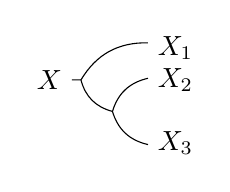
\begin{tikzpicture}[scale=0.8]
	\path (0,0) node (X) {$X$} 
	++ (0.5,0) coordinate (copy0)
	+ (1.5,0.5) node (X1) {$\RV{X}_1$}
	++ (0.5,-0.5) coordinate (copy1)
	+(1,0.5) node (X2) {$\RV{X}_2$}
	+(1,-0.5) node (X3) {$\RV{X}_3$};
	\draw (X) -- (copy0) to [bend left] (X1) (copy0) to [bend right] (copy1) to [bend left] (X2) (copy1) to [bend right] (X3);
	\end{tikzpicture}
	=
	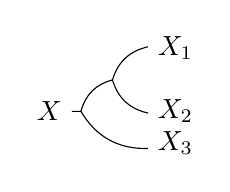
\begin{tikzpicture}[scale=0.8]
	\path (0,0) node (X) {$X$} 
	++ (0.5,0) coordinate (copy0)
	+ (1.5,-0.5) node (X1) {$\RV{X}_3$}
	++ (0.5,0.5) coordinate (copy1)
	+(1,0.5) node (X2) {$\RV{X}_1$}
	+(1,-0.5) node (X3) {$\RV{X}_2$};
	\draw (X) -- (copy0) to [bend right] (X1) (copy0) to [bend left] (copy1) to [bend left] (X2) (copy1) to [bend right] (X3);
	\end{tikzpicture}
	:=
	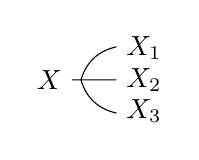
\begin{tikzpicture}[scale=0.8]
	\path (0,0) node (X) {$X$} 
	++ (0.5,0) coordinate (copy0)
	+ (1,0.5) node (X1) {$\RV{X}_1$}
	+(1,0) node (X2) {$\RV{X}_2$}
	+(1,-0.5) node (X3) {$\RV{X}_3$};
	\draw (X) -- (copy0) to [bend left] (X1) (copy0) to (X2) (copy0) to [bend right] (X3);
	\end{tikzpicture}\label{eq:ccom1}
\end{align}

\begin{align}
	\begin{tikzpicture}[scale=0.8]
	\path (0,0) node (X) {$X$}
	++(0.5,0) coordinate (copy0)
	+ (1,0.5) node (S) {}
	+(1,-0.5) node (X1) {$\RV{X}$};
	\draw (X) -- (copy0) to [bend right] (X1);
	\draw[-{Rays [n=8]}] (copy0) to [bend left] (S);
	\end{tikzpicture}
	= 
	\begin{tikzpicture}[scale=0.8]
	\path (0,0) node (X) {$X$}
	++(0.5,0) coordinate (copy0)
	+ (1,-0.5) node (S) {}
	+(1,0.5) node (X1) {$\RV{X}$};
	\draw (X) -- (copy0) to [bend left] (X1);
	\draw[-{Rays [n=8]}] (copy0) to [bend right] (S);
	\end{tikzpicture}
	=
	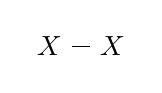
\begin{tikzpicture}[scale=0.8]
	\path (0,0) node (X) {$X$}
	++ (1,0) node (X1) {$\RV{X}$};
	\draw (X) -- (X1);
	\end{tikzpicture}\label{eq:ccom2}
\end{align}

\begin{align}
	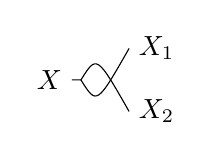
\begin{tikzpicture}[scale=0.8]
	\path (0,0) node (X) {$X$}
	++(0.5,0) coordinate (copy0)
	+ (1.2,0.5) node (X2) {$\RV{X}_1$}
	+(1.2,-0.5) node (X1) {$\RV{X}_2$};
	\draw (X) -- (copy0) .. controls (0.75,0.4) .. (X1.west);
	\draw (copy0) .. controls (0.75,-0.4) .. (X2.west);
	\end{tikzpicture}
=
	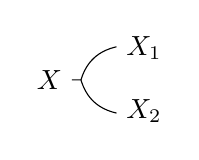
\begin{tikzpicture}[scale=0.8]
	\path (0,0) node (X) {$X$}
	++(0.5,0) coordinate (copy0)
	+ (1,0.5) node (X2) {$\RV{X}_1$}
	+(1,-0.5) node (X1) {$\RV{X}_2$};
	\draw (X) -- (copy0) to [bend right] (X1);
	\draw (copy0) to [bend left] (X2);
	\end{tikzpicture}\label{eq:ccom3}
\end{align}

The discard map $\stopper{0.2}$ can ``fall through'' any Markov kernel:

\begin{align}
\begin{tikzpicture}
\path (0,0) node (X) {$X$}
++(0.7,0) node[kernel] (A) {$\mathbf{A}$}
++(0.7,0) node (S) {};
\draw (X) -- (A);
\draw[-{Rays [n=8]}] (A) -- (S);
\end{tikzpicture}
= 
\begin{tikzpicture}
\path (0,0) node (X) {$X$}
++(0.7,0) node (S) {};
\draw[-{Rays [n=8]}] (X) -- (S);
\end{tikzpicture}\label{eq:termobj1}
\end{align}

Combining \ref{eq:ccom2} and \ref{eq:termobj1} we can derive the following: integrating $\mathbf{A}:X\to \Delta(\mathcal{Y})$ with respect to $\mu\in\Delta(\mathcal{X})$ and then discarding the output of $\mathbf{A}$ leaves us with $\mu$:

\begin{align}
\begin{tikzpicture}
\path (0,0) node[dist] (mu) {$\mu$}
++ (1,0) coordinate (copy0)
+ (1.4,0.5) node (X) {$\RV{X}$}
++ (0.7,-0.5) node[kernel] (A) {$\mathbf{A}$}
++(0.7,0) node (Y) {};
\draw (mu)--(copy0);
\draw (copy0) to [bend left] (X);
\draw[-{Rays [n=8]}] (copy0) to [bend right] (A) (A) -- (Y);
\end{tikzpicture}
= 
\begin{tikzpicture}
\path (0,0) node[dist] (mu) {$\mu$}
++ (1,0) coordinate (copy0)
+ (1.2,0.5) node (X) {$\RV{X}$}
++ (0.4,-0.3) coordinate (A)
++(0.1,0) node (Y) {};
\draw (mu)--(copy0);
\draw (copy0) to [bend left] (X);
\draw[-{Rays [n=8]}] (copy0) to [bend right] (A) (A) -- (Y);
\end{tikzpicture}
=
\begin{tikzpicture}
\path (0,0) node[dist] (mu) {$\mu$}
++ (1,0) node (X) {$\RV{X}$};
\draw (mu)--(X);
\end{tikzpicture}
\end{align}

In elementary notation, this is equivalent to the fact that, for all $B\in \mathcal{X}$, $\int_B \mathbf{A}(x;B)d\mu(x) = \mu(B)$.

\paragraph{Disintegraion and Bayesian Inversion}

A key reason for introducing the 

% \begin{align}
% \begin{tikzpicture}
% \path (0,0) node[dist] (mu) {$\mu$}
% ++ (1,0) coordinate (copy0)
% + (1.2,0.5) node (X) {$\RV{X}$}
% ++ (0.5,-0.5) node[kernel] (A) {$\mathbf{A}$}
% ++(0.7,0) node (Y) {$\RV{Y}$};
% \draw (mu)--(copy0);
% \draw (copy0) to [bend left] (X);
% \draw (copy0) to [bend right] (A) (A) -- (Y);
% \end{tikzpicture}\qquad
% \begin{tikzpicture}
% \path (0,0) node[dist] (mu) {$\mu$}
% ++ (1,0) coordinate (copy0)
% + (1.2,0.5) node (X) {$\RV{X}$}
% ++ (0.5,-0.5) node[kernel] (A) {$\mathbf{A}$}
% ++(0.7,0) node (Y) {};
% \draw (mu)--(copy0);
% \draw (copy0) to [bend left] (X);
% \draw[-{Rays [n=8]}] (copy0) to [bend right] (A) (A) -- (Y);
% \end{tikzpicture}=
% \begin{tikzpicture}
% \path (0,0) node[dist] (MU) {$\mu$}
% + (0.5,0) node (X) {$\RV{X}$};
% \draw (MU) -- (X);
% \end{tikzpicture}\label{eq:jdist}
% \end{align}


